
\providecommand{\rvAinc}{\vec{\mathcal{A}}}%
\providecommand{\rvAdec}{\overleftarrow{\mathcal{A}}}%
\providecommand{\wlim}{\operatorname{lim}}%
\providecommand{\wcolim}{\operatorname{colim}}%

\section{作为胞腔复形的 Reedy 范畴}\label{sec:reedy-categories-as-cell-complexes}

在本节中，我们描述一种承载于某些小范畴 $\mathcal{A}$ 之上的结构；Reedy 最先
利用这种结构来证明关于以 $\mathcal{A}$ 为标的图表\trCategory{}的种种同伦论
结果 \cite{bib99}。我们的首要例子——序数范畴 $\boldsymbol{\Delta}_+$、逆范畴、
它们的反范畴，以及这些范畴的乘积——全都是如 Daniel Kan 所定义的（严格的）%
\emph{Reedy \trCategory}\footnote{有关这一定义的标准书面文献——规范的模型范畴
教科书 \cite{bib55} 与 \cite{bib57} 所引用者——本是后来成为 \cite{bib39} 之书
的一部早期草稿；不过，等到这部手稿付印之时，它反倒转而引用上述文献，以便
「综述 Reedy 范畴这一概念」。}，因此我们把注意力限定于这一特殊情形。%
\footnote{这一理论已被 Berger 与 Moerdijk 有益地加以扩充，使之涵盖「广义
Reedy 范畴」——其中容许对象拥有非恒同的自同构 \cite{bib12}。}我们的讲述
沿循 \cite{bib107}。

\begin{definition}[Reedy 结构]\label{def:reedy-structure}
小\trCategory{} $\mathcal{A}$ 上的一个\textbf{Reedy 结构}（Reedy structure）
由一个\textbf{度函数}（degree function）$\mathrm{deg}\colon\mathrm{obj}\mathcal{A}\to\omega$ 连同\textbf{宽子范畴}（wide subcategories）的一对
$\rvAinc$ 与 $\rvAdec$——分别由\textbf{升度}（degree-increasing）与\textbf{降度}
（degree-decreasing）箭头组成——所构成，使得
\begin{enumerate}[label=(\roman*)]
\item 对 $\rvAinc$ 中每个非恒同态射，其定义域的度数严格小于其陪域的度数；
  而对 $\rvAdec$ 中每个非恒同态射，其定义域的度数严格大于其陪域的度数%
  \yizhu{原书于此印作 the degree of its domain，按对偶文义疑为 codomain 之误，
  此处径改。}；
\item $\mathcal{A}$ 中的每个态射 $f$ 都可以唯一地分解为
\begin{rveq}\label{eq:reedy-factorization}
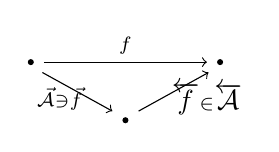
\begin{tikzpicture}[x=1.9em,y=1.5em]
  \fill (0,1.4) circle (1.1pt);
  \fill (3.6,1.4) circle (1.1pt);
  \fill (1.8,0) circle (1.1pt);
  \draw[->] (0.25,1.4) -- (3.35,1.4);
  \node at (1.8,1.8) {$\scriptstyle f$};
  \draw[->] (0.22,1.15) -- (1.55,0.22);
  \node at (0.55,0.52) {$\scriptstyle\rvAinc\ni\vec{f}$};
  \draw[->] (2.05,0.22) -- (3.38,1.15);
  \node at (3.35,0.52) {$\scriptstyle\overleftarrow{f}\in\rvAdec$};
\end{tikzpicture}
\end{rveq}
\end{enumerate}
\end{definition}

公理 (i) 蕴含 $\rvAinc\cap\rvAdec=\mathrm{obj}(\mathcal{A})$，而这两条条件
合在一起则蕴含 $\mathcal{A}$ 不含非恒同的自同构（见\cref{ex:reedy-isomorphism-identity}）。

\begin{example}\label{exa:inverse-category-reedy}
任何逆范畴 $\mathcal{J}$（见\cref{def:inverse-category}）都是一个 Reedy 范畴，
此时取 $\vec{\mathcal{J}}=\mathcal{J}$ 而 $\overleftarrow{\mathcal{J}}=\mathrm{obj}\mathcal{J}$。
反之，任何满足 $\mathcal{A}=\rvAinc$ 的 Reedy 范畴 $\mathcal{A}$ 都是一个逆
范畴，在此情形下，其度\emph{函数}可扩充为一个反映恒同箭头的度\emph{函子}。
\end{example}

\begin{example}\label{exa:delta-plus-reedy}
\trCategory{} $\boldsymbol{\Delta}_+$ 是一个 Reedy 范畴，其中取
$\vec{\boldsymbol{\Delta}}_+$ 为\trMonomorphism{}组成的子范畴、取
$\overleftarrow{\boldsymbol{\Delta}}_+$ 为\trEpimorphism{}组成的子范畴。在此，
方便的做法是利用序同构 $\mathbb{1}+\omega\cong\omega$ 来定义 $\mathrm{deg}[n]:=n$。
子范畴 $\boldsymbol{\Delta}$、$\boldsymbol{\Delta}_\top$ 与
$\boldsymbol{\Delta}_\bot$ 都继承类似的 Reedy 范畴结构。
\end{example}

\begin{remark}\label{rem:opposite-reedy}
若 $\mathcal{A}$ 是一个 Reedy 范畴，则 $\mathcal{A}^{\mathrm{op}}$ 亦是：其
Reedy 结构拥有同一度函数，但升度箭头与降度箭头互换。特别地，%
\cref{exa:inverse-category-reedy} 中的诸 Reedy 范畴对偶地定义了\textbf{正范畴}
（direct categories），后者配有反映恒同箭头的\trFunctor{}
$\mathrm{deg}\colon\mathcal{A}\to\omega$。
\end{remark}

\begin{example}\label{exa:product-reedy}
若 $\mathcal{A}$ 与 $\mathcal{B}$ 是 Reedy 范畴，则 $\mathcal{A}\times\mathcal{B}$
亦是，其度数为 $\mathrm{deg}(a,b):=\mathrm{deg}(a)+\mathrm{deg}(b)$
（见\cref{ex:product-reedy-category}）。
\end{example}

在本节余下的部分中，我们固定一个 Reedy 范畴 $\mathcal{A}$。我们把唯一分解
\eqref{eq:reedy-factorization} 称作映射 $f$ 的\textbf{Reedy 分解}（Reedy
factorization），并把对象 $\mathrm{cod}\,\vec{f}=\mathrm{dom}\,\overleftarrow{f}$
的度数称作 $f$ 的\textbf{度数}（degree）。我们的下一个目标是证明：
\begin{enumerate}[label=(\roman*)]
\item $f$ 的度数是 $f$ 可经由之分解的对象的最小度数。
\item $f$ 经由具有这一度数的对象之分解唯有 Reedy 分解。
\end{enumerate}

为证明这些论断，试考虑范畴
$\mathcal{F}act f:=(a/\mathcal{A})_{/f}\cong f/(\mathcal{A}_{/b})$，
其对象为 $f$ 的分解 $a\xrightarrow{\ g\ }c\xrightarrow{\ h\ }b$，其态射
$h\cdot g\to h'\cdot g'$ 是使得前侧三角形
\begin{center}
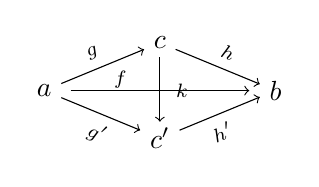
\begin{tikzpicture}[x=1.9em,y=1.5em]
  \node (c) at (2.2,2.3) {$c$};
  \node (a) at (0,1.15) {$a$};
  \node (b) at (4.4,1.15) {$b$};
  \node (c2) at (2.2,0) {$c'$};
  \draw[->] (a) -- (c) node[pos=0.45,above,sloped]{$\scriptstyle g$};
  \draw[->] (c) -- (b) node[pos=0.55,above,sloped]{$\scriptstyle h$};
  \draw[->] (0.5,1.15) -- (3.9,1.15);
  \node at (1.45,1.42) {$\scriptstyle f$};
  \draw[->] (2.2,1.95) -- (2.2,0.4);
  \node at (2.62,1.15) {$\scriptstyle k$};
  \draw[->] (a) -- (c2) node[pos=0.55,below,sloped]{$\scriptstyle g'$};
  \draw[->] (c2) -- (b) node[pos=0.45,below,sloped]{$\scriptstyle h'$};
\end{tikzpicture}
\end{center}
得以交换的映射 $k\colon c\to c'$。记
$\mathcal{F}act_{\leq n}f\subset\mathcal{F}act f$ 为经由度数至多为 $n$ 的对象
之分解所组成的全子范畴。

\begin{lemma}\label{lem:fact-connected}
范畴 $\mathcal{F}act f$ 是连通的，且每个全子范畴
$\mathcal{F}act_{\leq n}f$ 要么为空要么连通。使 $\mathcal{F}act_{\leq n}f$
非空的最小 $n$ 即 $f$ 的度数，并且
$\mathcal{F}act_{\leq\mathrm{deg}(f)}f\cong\mathbb{1}$。
\end{lemma}

\begin{proof}
考察 $h\cdot g\in\mathcal{F}act f$ 及其诸 Reedy 分解：
\begin{rveq}\label{eq:fact-zigzag}
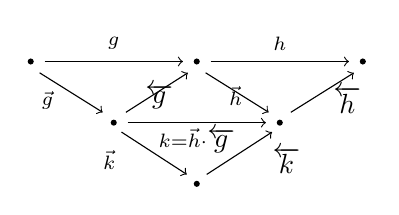
\begin{tikzpicture}[x=2.0em,y=1.7em]
  \fill (0,2.6) circle (1.1pt);
  \fill (3.0,2.6) circle (1.1pt);
  \fill (6.0,2.6) circle (1.1pt);
  \fill (1.5,1.3) circle (1.1pt);
  \fill (4.5,1.3) circle (1.1pt);
  \fill (3.0,0) circle (1.1pt);
  \draw[->] (0.25,2.6) -- (2.75,2.6);
  \node at (1.5,2.98) {$\scriptstyle g$};
  \draw[->] (3.25,2.6) -- (5.75,2.6);
  \node at (4.5,2.98) {$\scriptstyle h$};
  \draw[->] (0.16,2.36) -- (1.3,1.52);
  \node at (0.3,1.78) {$\scriptstyle\vec{g}$};
  \draw[->] (1.72,1.52) -- (2.84,2.36);
  \node at (2.32,1.86) {$\scriptstyle\overleftarrow{g}$};
  \draw[->] (3.16,2.36) -- (4.3,1.52);
  \node at (3.7,1.86) {$\scriptstyle\vec{h}$};
  \draw[->] (4.7,1.52) -- (5.84,2.36);
  \node at (5.72,1.78) {$\scriptstyle\overleftarrow{h}$};
  \draw[->] (1.75,1.3) -- (4.25,1.3);
  \node at (3.0,0.92) {$\scriptstyle k=\vec{h}\cdot\overleftarrow{g}$};
  \draw[->] (1.64,1.1) -- (2.82,0.2);
  \node at (1.42,0.5) {$\scriptstyle\vec{k}$};
  \draw[->] (3.18,0.2) -- (4.36,1.1);
  \node at (4.62,0.5) {$\scriptstyle\overleftarrow{k}$};
\end{tikzpicture}
\end{rveq}
这样，我们便在 $\mathcal{F}act f$ 中定义了一条连接 $h\cdot g$ 与
$\overleftarrow{h}\,\overleftarrow{k}\cdot\vec{k}\,\vec{g}$ 的态射之字形链，
而由公理 (ii)，后者必为 $f$ 的 Reedy 分解。这表明 $\mathcal{F}act f$ 是连通的。

此外，公理 (i) 蕴含 $\mathrm{cod}(g)=\mathrm{dom}(h)$ 的度数至少是 $f$ 的
度数。特别地，若 $h\cdot g\in\mathcal{F}act_{\leq n}f$，则
\eqref{eq:fact-zigzag} 中的每个分解亦然，这就证明了 $\mathcal{F}act_{\leq n}f$
在非空时必定连通。这一图式还表明：每个非空范畴 $\mathcal{F}act_{\leq n}f$
都包含 Reedy 分解。于是，使之非空的最小 $n$ 便是 $f$ 的度数。

最后，若 $\mathrm{cod}(g)=\mathrm{dom}(h)$ 的度数等于 $f$ 的度数，则
$\overleftarrow{g}$ 与 $\vec{h}$（以及 $\vec{k}$ 与 $\overleftarrow{k}$）必为
恒同，由此我们推得 $g\in\rvAinc$ 且 $h\in\rvAdec$；也就是说，$h\cdot g$ 就是
Reedy 分解。于是，正如所断言的，
$\mathcal{F}act_{\leq\mathrm{deg}(f)}f\cong\mathbb{1}$ 是\trTerminal{}范畴。
\end{proof}

\cref{lem:fact-connected} 将被用来为 hom 双函子确立一种「胞腔分解」（cellular
decomposition）；这一 hom 双函子在别处记作 $\mathcal{A}(-,-)$，而在此处则
缩记为 $\mathcal{A}\in\mathcal{S}et^{\mathcal{A}^{\mathrm{op}}\times\mathcal{A}}$。
Reedy 结构使我们得以把双函子 $\mathcal{A}$ 呈现为\cref{def:cell-complex} 意义下
的一个胞腔复形，即一个由具有特定形状的基本「\trCell{}」之余积的推出构成的序列
复合。\cref{lem:fact-connected} 蕴含：度数至多为 $n$ 的箭头组成的子集可以
组装成 hom 双函子的一个\emph{子函子}。

\begin{definition}[hom 双函子的 $n$-骨架]\label{def:n-skeleton-hom-bifunctor}
对任何 Reedy 范畴 $\mathcal{A}$，\textbf{$n$-骨架}（$n$-skeleton）是度数至多
为 $n$ 的箭头组成的子函子
\[ \mathrm{sk}_n\mathcal{A}\hookrightarrow\mathcal{A}
   \in\mathcal{S}et^{\mathcal{A}^{\mathrm{op}}\times\mathcal{A}} \]
\end{definition}

存在显然的包含 $\mathrm{sk}_{n-1}\mathcal{A}\hookrightarrow\mathrm{sk}_n\mathcal{A}$。
序列
\[ \varnothing\hookrightarrow\mathrm{sk}_0\mathcal{A}\hookrightarrow\cdots
   \hookrightarrow\mathrm{sk}_{n-1}\mathcal{A}\hookrightarrow\mathrm{sk}_n\mathcal{A}
   \hookrightarrow\cdots\hookrightarrow\wcolim\mathrm{sk}_n\mathcal{A}\cong\mathcal{A} \]
的余极限就是 hom 双函子 $\mathcal{A}$。度数为 $n$ 的态射首次出现于
$\mathrm{sk}_n\mathcal{A}$ 中。剩下的工作是把每个包含
$\mathrm{sk}_{n-1}\mathcal{A}\hookrightarrow\mathrm{sk}_n\mathcal{A}$ 表述为
基本「\trCell{}」之余积的一个推出，这种基本「\trCell{}」我们即刻描述。

外部（逐点）积定义了一个双函子
$\square\colon\mathcal{S}et^{\mathcal{A}}\times\mathcal{S}et^{\mathcal{A}^{\mathrm{op}}}\to\mathcal{S}et^{\mathcal{A}^{\mathrm{op}}\times\mathcal{A}}$。对任何
$a\in\mathcal{A}$，都存在一个自然的「复合」映射
$\circ\colon\mathcal{A}_a\square\mathcal{A}^{a}\to\mathcal{A}$，其定义域是反变
可表示函子 $\mathcal{A}^{a}$ 与协变可表示函子 $\mathcal{A}_a$ 的外部积；此处
我们以 $\mathcal{A}^{a}$ 缩记 $\mathcal{A}(-,a)$、以 $\mathcal{A}_a$ 缩记
$\mathcal{A}(a,-)$。由\cref{lem:fact-connected}，经由一个度数为 $n$ 的对象 $a$
而分解的任何一对映射的复合都落于 $\mathrm{sk}_n\mathcal{A}$ 中，这就定义了
一个映射：
\[ \coprod_{\mathrm{deg}(a)=n}\mathcal{A}_a\square\mathcal{A}^{a}
   \xrightarrow{\ \circ\ }\mathrm{sk}_n\mathcal{A} \]

我们的下一项任务是描述定义域中经由
$\mathrm{sk}_{n-1}\mathcal{A}\hookrightarrow\mathrm{sk}_n\mathcal{A}$ 而分解的
那个子函子；为此我们需要一些新记号。

\begin{definition}[可表示函子的边缘]\label{def:boundary-representables}
若 $a\in\mathcal{A}$ 的度数为 $n$，则写作
\[ \begin{gathered}
\partial\mathcal{A}_a:=\mathrm{sk}_{n-1}\mathcal{A}_a
   \qquad\in\mathcal{S}et^{\mathcal{A}}\qquad\text{以及}\\
\partial\mathcal{A}^{a}:=\mathrm{sk}_{n-1}\mathcal{A}^{a}
   \qquad\in\mathcal{S}et^{\mathcal{A}^{\mathrm{op}}}.
\end{gathered} \]
\end{definition}

由\cref{lem:fact-connected}，$\partial\mathcal{A}_a\hookrightarrow\mathcal{A}_a$
是 $\mathcal{A}$ 中定义域为 $a$ 且\emph{不}居于 $\rvAinc$ 的箭头组成的子函子，
而 $\partial\mathcal{A}^{a}\hookrightarrow\mathcal{A}^{a}$ 是陪域为 $a$
且\emph{不}居于 $\rvAdec$ 的箭头组成的子函子。

特别地，外部\trLeibnizProduct
\[ \mathcal{A}_a\square\partial\mathcal{A}^{a}
   \cup_{\partial\mathcal{A}_a\square\partial\mathcal{A}^{a}}
   \partial\mathcal{A}_a\square\mathcal{A}^{a}
   \xhookrightarrow{\ (\partial\mathcal{A}_a\hookrightarrow\mathcal{A}_a)
   \mathbin{\widehat{\square}}(\partial\mathcal{A}^{a}\hookrightarrow\mathcal{A}^{a})\ }
   \mathcal{A}_a\square\mathcal{A}^{a} \]
定义了由满足 $\mathrm{dom}\,h=\mathrm{cod}\,g=a$ 的态射对 $h\cdot g$ 组成的
子函子，其中态射 $g$ 与 $h$ 至少有一个的度数小于 $a$ 的度数。

\begin{proposition}\label{prop:sk-square-pullback-pushout}
所展示的交换方块在 $\mathcal{S}et^{\mathcal{A}^{\mathrm{op}}\times\mathcal{A}}$
中既是一个拉回又是一个推出。
\begin{rveq}\label{eq:sk-square}
\begin{tikzpicture}[x=1.7em,y=1.6em]
  \node (TL) at (0,1.55) {$\displaystyle\coprod_{\mathrm{deg}(a)=n}\partial\mathcal{A}_a\square\mathcal{A}^{a}\cup\mathcal{A}_a\square\partial\mathcal{A}^{a}$};
  \node (TR) at (8.6,1.55) {$\displaystyle\coprod_{\mathrm{deg}(a)=n}\mathcal{A}_a\square\mathcal{A}^{a}$};
  \node (BL) at (0,0) {$\mathrm{sk}_{n-1}\mathcal{A}$};
  \node (BR) at (8.6,0) {$\mathrm{sk}_n\mathcal{A}$};
  \draw[right hook->] (TL) -- (TR);
  \draw[->] (0,1.1) -- (0,0.42);
  \node at (0.42,0.76) {$\scriptstyle\circ$};
  \draw[->] (8.6,1.1) -- (8.6,0.42);
  \node at (9.02,0.76) {$\scriptstyle\circ$};
  \draw[->] (BL) -- (BR);
\end{tikzpicture}
\end{rveq}
\end{proposition}

\eqref{eq:sk-square} 是拉回这一事实，将被用来便利其亦为推出之证明。

\begin{proof}
该拉回中的一个元素由 $f\in\mathrm{sk}_{n-1}\mathcal{A}$ 连同 $f=h\cdot g$
经由一个度数为 $n$ 的对象 $a$ 的一个分解构成。若 $h$ 与 $g$ 二者的度数都是
$n$，则\cref{lem:fact-connected} 告诉我们 $h\cdot g$ 是一个 Reedy 分解，这与
$f$ 的度数至多为 $n-1$ 的事实相矛盾。所以我们必有 $h\in\partial\mathcal{A}_a$
或 $g\in\partial\mathcal{A}^{a}$，这就告诉我们：从 \eqref{eq:sk-square} 左上角
出发的映射满映到该拉回上。由于顶行的水平映射是单的，该比较映射因而是一个
同构；也就是说，\eqref{eq:sk-square} 是一个拉回方块。

为证它是推出，现在只需证明右侧的竖直映射在
$\mathrm{sk}_{n-1}\mathcal{A}\hookrightarrow\mathrm{sk}_n\mathcal{A}$ 的补上是
一对一的。这由\cref{lem:fact-connected} 得出，后者论证了任何度数为 $n$ 的态射
都拥有经由该度数之对象的一个唯一分解，即其 Reedy 分解。
\end{proof}

作为\cref{prop:sk-square-pullback-pushout} 的推论，hom 双函子 $\mathcal{A}$
容有一个作为胞腔复形的典范呈现。

\begin{theorem}\label{thm:canonical-cell-complex}
包含 $\varnothing\hookrightarrow\mathcal{A}\in\mathcal{S}et^{\mathcal{A}^{\mathrm{op}}\times\mathcal{A}}$ 拥有一个作为胞腔
复形的典范呈现：
\begin{center}
\begin{tikzpicture}[x=1.25em,y=1.6em]
  \node (TL) at (0,1.7) {$\displaystyle\coprod_{\mathrm{deg}(a)=n}\partial\mathcal{A}_a\square\mathcal{A}^{a}\cup\mathcal{A}_a\square\partial\mathcal{A}^{a}$};
  \node (TR) at (8.8,1.7) {$\displaystyle\coprod_{\mathrm{deg}(a)=n}\mathcal{A}_a\square\mathcal{A}^{a}$};
  \draw[right hook->] (TL) -- (TR);
  \draw[->] (0,1.22) -- (0,0.5);
  \node at (0.4,0.86) {$\scriptstyle\circ$};
  \draw[->] (8.8,1.22) -- (8.8,0.5);
  \node at (9.2,0.86) {$\scriptstyle\circ$};
  \node (E) at (-9.6,0) {$\varnothing$};
  \node (S0) at (-7.2,0) {$\mathrm{sk}_0\mathcal{A}$};
  \node (D1) at (-5.0,0) {$\cdots$};
  \node (BL) at (0,0) {$\mathrm{sk}_{n-1}\mathcal{A}$};
  \node (BR) at (8.8,0) {$\mathrm{sk}_n\mathcal{A}$};
  \node (D2) at (10.9,0) {$\cdots$};
  \node (CL) at (14.6,0) {$\wcolim_n\mathrm{sk}_n\mathcal{A}\cong\mathcal{A}$};
  \draw[right hook->] (-9.2,0) -- (-8.3,0);
  \draw[dotted,->] (-6.1,0) -- (-5.55,0);
  \draw[dotted,->] (-4.45,0) -- (-1.8,0);
  \draw[right hook->] (1.2,0) -- (7.9,0);
  \node at (8.15,0.34) {$\scriptstyle\lrcorner$};
  \draw[dotted,->] (9.7,0) -- (10.35,0);
  \draw[->] (11.5,0) -- (11.9,0);
\end{tikzpicture}
\end{center}
也就是说，它是诸\trCell{}之余积的推出的一个序列复合，而诸\trCell{}定义为
外部\trLeibnizProduct
\[ (\partial\mathcal{A}_a\hookrightarrow\mathcal{A}_a)\mathbin{\widehat{\square}}
   (\partial\mathcal{A}^{a}\hookrightarrow\mathcal{A}^{a}), \]
其中 $\mathcal{A}$ 的每个度数为 $n$ 的对象 $a$ 所对应的\trCell{}在第 $n$
阶段粘合。
\end{theorem}

作为\cref{thm:canonical-cell-complex} 的推论，任何态射
$f\in\mathcal{M}^{\mathcal{A}}$ 自身就是一个胞腔复形：$\mathcal{A}$ 的胞腔
分解经由取加权余极限而被转译为 $f$ 的一个胞腔分解。若改为取加权极限，则把
$\mathcal{A}$ 的胞腔分解转变为 $f$ 的一个「Postnikov 呈现」（Postnikov
presentation）——即作为可数塔之极限的、由特定映射之积的拉回构成的一座塔。
这类结果正是 \cite{bib107} 那句口号——「一切尽在权重之中」——的范例。在证明
这一推论之前，我们需要一些记号，以记写作为基本\trCell{}与基本层登场的那些映射。

\begin{definition}[锁存对象与匹配对象]\label{def:latching-matching-objects}
设 $a\in\mathcal{A}$。\trDiagram{} $X\in\mathcal{M}^{\mathcal{A}}$ 在 $a$ 处的
\textbf{锁存对象}（latching object）与\textbf{匹配对象}分别定义为以适当变式的
边缘可表示函子加权所得的余极限与极限：
\[ L^{a}X:=\wcolim_{\partial\mathcal{A}^{a}}X\qquad
   M^{a}X:=\wlim_{\partial\mathcal{A}_a}X. \]
\end{definition}

边缘包含 $\partial\mathcal{A}^{a}\hookrightarrow\mathcal{A}^{a}$ 与
$\partial\mathcal{A}_a\hookrightarrow\mathcal{A}_a$ 诱导出\textbf{\trLatchingMap}
（latching map）与\textbf{匹配映射} $\ell^{a}\colon L^{a}X\to X^{a}$ 与
$m^{a}\colon X^{a}\to M^{a}X$，其依据是附录 A 中的%
\cref{def:weighted-limit-colimit-axiomatic}(i) 的诸同构
$\wcolim_{\mathcal{A}^{a}}X\cong X^{a}\cong\wlim_{\mathcal{A}_a}X$。

\begin{definition}[相对锁存映射与相对匹配映射]\label{def:relative-latching-matching-maps}
自然变换 $f\colon X\to Y\in\mathcal{M}^{\mathcal{A}}$ 的\textbf{相对锁存映射}
（relative latching map）与\textbf{相对匹配映射}定义为 Leibniz 加权余极限与
加权极限
\[ \hat{\ell}^{a}f:=\widehat{\wcolim}_{\partial\mathcal{A}^{a}\hookrightarrow\mathcal{A}^{a}}f
   \qquad
   \hat{m}^{a}f:=\widehat{\wlim}_{\partial\mathcal{A}_a\hookrightarrow\mathcal{A}_a}f, \]
亦即由下列诸拉回与诸推出给出：
\begin{center}
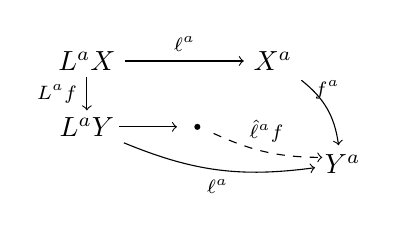
\begin{tikzpicture}[x=2.1em,y=1.7em]
  \node (LX) at (0,2.4) {$L^{a}X$};
  \node (Xa) at (3.2,2.4) {$X^{a}$};
  \node (LY) at (0,1.0) {$L^{a}Y$};
  \fill (1.9,1.0) circle (1.1pt);
  \node (Ya) at (4.4,0.2) {$Y^{a}$};
  \draw[->] (LX) -- (Xa) node[midway,above]{$\scriptstyle\ell^{a}$};
  \draw[->] (0,2.05) -- (0,1.35) node[midway,left]{$\scriptstyle L^{a}f$};
  \draw[->] (0.55,1.0) -- (1.55,1.0);
  \node at (2.42,1.32) {$\scriptstyle\lrcorner$};
  \draw[dashed,->] (2.18,0.86) to[bend right=12] node[pos=0.5,above]{$\scriptstyle\hat{\ell}^{a}f$} (4.05,0.35);
  \draw[->] (Xa) to[bend left=22] node[pos=0.5,above]{$\scriptstyle f^{a}$} (Ya);
  \draw[->] (LY) to[bend right=15] node[pos=0.5,below]{$\scriptstyle\ell^{a}$} (Ya);
\end{tikzpicture}
\qquad
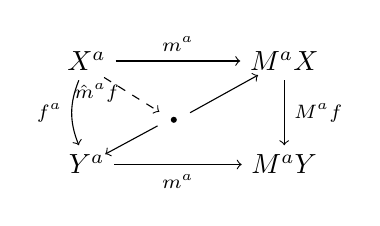
\begin{tikzpicture}[x=2.1em,y=1.7em]
  \node (Xa) at (0,2.4) {$X^{a}$};
  \node (MX) at (3.4,2.4) {$M^{a}X$};
  \fill (1.5,1.15) circle (1.1pt);
  \node (Ya) at (0,0.2) {$Y^{a}$};
  \node (MY) at (3.4,0.2) {$M^{a}Y$};
  \draw[->] (Xa) -- (MX) node[midway,above]{$\scriptstyle m^{a}$};
  \draw[dashed,->] (0.3,2.05) -- (1.25,1.32) node[pos=0.45,left]{$\scriptstyle\hat{m}^{a}f$};
  \draw[->] (1.78,1.3) -- (2.95,2.1);
  \node at (2.12,0.98) {$\scriptstyle\lrcorner$};
  \draw[->] (1.22,1.02) -- (0.32,0.42);
  \draw[->] (MX) -- (MY) node[midway,right]{$\scriptstyle M^{a}f$};
  \draw[->] (Ya) -- (MY) node[midway,below]{$\scriptstyle m^{a}$};
  \draw[->] (Xa) to[bend right=22] node[pos=0.5,left]{$\scriptstyle f^{a}$} (Ya);
\end{tikzpicture}
\end{center}
其中的映射为 $L^{a}f:=\wcolim_{\partial\mathcal{A}^{a}}f$ 与
$M^{a}f:=\wlim_{\partial\mathcal{A}_a}f$。
\end{definition}

\begin{notation}\label{not:sk-cosk-diagrams}
对任何\trDiagram{} $X\in\mathcal{M}^{\mathcal{A}}$，记
\[ \mathrm{sk}_nX:=\wcolim_{\mathrm{sk}_n\mathcal{A}}X\qquad\text{以及}\qquad
   \mathrm{cosk}_nX:=\wlim_{\mathrm{sk}_n\mathcal{A}}X \]
为把附录 A 中的\cref{ex:enriched-profunctor-weights} 的加权余极限与加权极限
双函子
\[ \wcolim_{--}\colon\mathcal{S}et^{\mathcal{A}^{\mathrm{op}}\times\mathcal{A}}
   \times\mathcal{M}^{\mathcal{A}}\to\mathcal{M}^{\mathcal{A}}
   \qquad\text{与}\qquad
   \wlim_{--}\colon(\mathcal{S}et^{\mathcal{A}^{\mathrm{op}}\times\mathcal{A}})^{\mathrm{op}}
   \times\mathcal{M}^{\mathcal{A}}\to\mathcal{M}^{\mathcal{A}} \]
施加于带权 $\mathrm{sk}_n\mathcal{A}$ 的\trDiagram{} $X$ 所得的结果。
\end{notation}

回顾为带余积与积的\trCategory{}所定义的集合张量
$\ast\colon\mathcal{S}et\times\mathcal{M}\to\mathcal{M}$ 与集合余张量
$\{,\}\colon\mathcal{S}et^{\mathrm{op}}\times\mathcal{M}\to\mathcal{M}$ 这两个%
\trBifunctor。

\begin{corollary}\label{cor:morphism-cell-complex}
设 $\mathcal{A}$ 是一个 Reedy 范畴，并设 $\mathcal{M}$ 完备且余完备。任何
态射 $f\colon X\to Y\in\mathcal{M}^{\mathcal{A}}$ 都是一个胞腔复形
\[ X\to
   X\cup_{\mathrm{sk}_0X}\mathrm{sk}_0Y\to\cdots\to
   X\cup_{\mathrm{sk}_{n-1}X}\mathrm{sk}_{n-1}Y\to
   X\cup_{\mathrm{sk}_nX}\mathrm{sk}_nY\to\cdots\to
   \wcolim\cong Y \]
其第 $n$ 阶段粘合以度数为 $n$ 的诸对象 $a$ 为标的诸\trCell
\[ (\partial\mathcal{A}_a\hookrightarrow\mathcal{A}_a)\mathbin{\widehat{\ast}}
   \hat{\ell}^{a}f \]
的余积，并且也是一座「Postnikov 塔」（Postnikov tower）
\[ \begin{gathered}
X\cong\lim\to\cdots\to
\mathrm{cosk}_nX\times_{\mathrm{cosk}_nY}Y\to\\
\mathrm{cosk}_{n-1}X\times_{\mathrm{cosk}_{n-1}Y}Y\to\cdots\to
\mathrm{cosk}_0X\times_{\mathrm{cosk}_0Y}Y\to Y
\end{gathered} \]
其第 $n$ 层是以度数为 $n$ 的诸对象 $a$ 为标的诸映射
\[ \{\partial\mathcal{A}^{a}\hookrightarrow\mathcal{A}^{a},\ \hat{m}^{a}f\} \]
之积。
\end{corollary}

\begin{proof}
这一对对偶结果可立即得到：只需把附录 A 中的\cref{ex:enriched-profunctor-weights}
的加权余极限与加权极限双函子
\[ \wcolim_{--}\colon\mathcal{S}et^{\mathcal{A}^{\mathrm{op}}\times\mathcal{A}}
   \times\mathcal{M}^{\mathcal{A}}\to\mathcal{M}^{\mathcal{A}}
   \qquad\text{以及}\qquad
   \wlim_{--}\colon(\mathcal{S}et^{\mathcal{A}^{\mathrm{op}}\times\mathcal{A}})^{\mathrm{op}}
   \times\mathcal{M}^{\mathcal{A}}\to\mathcal{M}^{\mathcal{A}} \]
施加于\cref{thm:canonical-cell-complex} 的诸胞腔复形呈现即可；并回想附录 A 中
的\cref{def:weighted-limit-colimit-axiomatic}(ii)：这两个双函子在权上都是
余连续的。

为看出 $f$ 的胞腔复形呈现具有所断言的形状，注意：对任何\trDiagram{}
$X\in\mathcal{M}^{\mathcal{A}}$ 与由 $U\in\mathcal{S}et^{\mathcal{A}}$ 及
$V\in\mathcal{S}et^{\mathcal{A}^{\mathrm{op}}}$ 的外部积所定义的权，都存在一个
自然\trIsomorphism{} $\wcolim_{U\square V}X\cong U\ast\wcolim_{V}X$，它可扩充
为诸\trLeibnizProduct{}之间的一个自然\trIsomorphism
（\cref{prop:leibniz-construction-preserves}(i)）。

由余 Yoneda 引理（coYoneda lemma），
$f\cong\wcolim_{\mathcal{A}}f\cong\widehat{\wcolim}_{\varnothing\hookrightarrow\mathcal{A}}f$。
由\cref{prop:leibniz-construction-preserves}(vii)，Leibniz 加权余极限函子
$\wcolim_{-}f$ 保持胞腔结构。于是，$f$ 容有一个作为胞腔复形的典范呈现，其诸%
\trCell{}为
\[ \widehat{\wcolim}_{(\partial\mathcal{A}_a\hookrightarrow\mathcal{A}_a)
   \mathbin{\widehat{\square}}(\partial\mathcal{A}^{a}\hookrightarrow\mathcal{A}^{a})}f
   \cong(\partial\mathcal{A}_a\hookrightarrow\mathcal{A}_a)\mathbin{\widehat{\ast}}
   \widehat{\wcolim}_{\partial\mathcal{A}^{a}\hookrightarrow\mathcal{A}^{a}}f
   \cong(\partial\mathcal{A}_a\hookrightarrow\mathcal{A}_a)\mathbin{\widehat{\ast}}
   \hat{\ell}^{a}f. \]
\end{proof}

这一呈现对 Reedy 范畴 $\boldsymbol{\Delta}^{\mathrm{op}}$ 而言最为眼熟。此处
我们以 $\boldsymbol{\Delta}^{n}$ 表示标准 $n$-\trSimplex{} $\Delta[n]$、以
$\partial\boldsymbol{\Delta}^{n}$ 表示其边缘——这些是文献中通行的记号约定，
且与\cref{def:boundary-representables} 的记法相容。

\begin{example}\label{exa:skeletal-filtration}
取值于任何余完备\trCategory{}的单纯对象 $Y$ 容有一个骨架过滤
（skeletal filtration）
\[ \varnothing\to\mathrm{sk}_0Y\to\cdots\to
   \mathrm{sk}_{n-1}Y\to\mathrm{sk}_nY\to\cdots\to
   \wcolim_n\mathrm{sk}_nY\cong Y \]
其中从阶段 $n-1$ 到阶段 $n$ 的一步由一个推出给出
\begin{center}
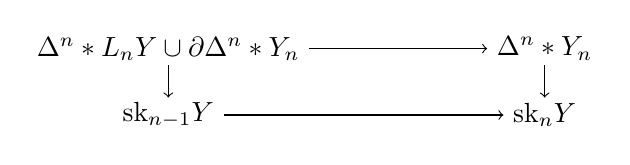
\begin{tikzpicture}[x=2.0em,y=1.5em]
  \node (TL) at (0,1.6) {$\boldsymbol{\Delta}^{n}\ast L_nY\cup\partial\boldsymbol{\Delta}^{n}\ast Y_n$};
  \node (TR) at (6.8,1.6) {$\boldsymbol{\Delta}^{n}\ast Y_n$};
  \node (BL) at (0,0) {$\mathrm{sk}_{n-1}Y$};
  \node (BR) at (6.8,0) {$\mathrm{sk}_nY$};
  \draw[->] (TL) -- (TR);
  \draw[->] (0,1.2) -- (0,0.42);
  \draw[->] (6.8,1.2) -- (6.8,0.42);
  \draw[->] (BL) -- (BR);
  \node at (6.15,0.36) {$\scriptstyle\lrcorner$};
\end{tikzpicture}
\end{center}
其中 $L_nY\to Y_n$ 是「退化 $n$-单纯形」组成的对象。

把\trYonedaEmbedding{}视作一个单纯对象
$\boldsymbol{\Delta}\in(\mathcal{S}et^{\boldsymbol{\Delta}})^{\boldsymbol{\Delta}^{\mathrm{op}}}$，
上式便特化为\cref{thm:canonical-cell-complex} 的那个 hom 双函子的「典范胞腔
复形呈现」
\begin{center}
\begin{tikzpicture}[x=1.6em,y=1.5em]
  \node (TL) at (0,1.7) {$\boldsymbol{\Delta}^{n}\times\partial\boldsymbol{\Delta}_n\cup\partial\boldsymbol{\Delta}^{n}\times\boldsymbol{\Delta}_n$};
  \node (TR) at (6.2,1.7) {$\boldsymbol{\Delta}^{n}\times\boldsymbol{\Delta}_n$};
  \draw[right hook->] (TL) -- (TR);
  \draw[->] (0,1.28) -- (0,0.5);
  \draw[->] (6.2,1.28) -- (6.2,0.5);
  \node (E) at (-6.0,0) {$\varnothing$};
  \node (D1) at (-4.4,0) {$\cdots$};
  \node (BL) at (0,0) {$\mathrm{sk}_{n-1}\boldsymbol{\Delta}$};
  \node (BR) at (6.2,0) {$\mathrm{sk}_n\boldsymbol{\Delta}$};
  \node (D2) at (8.3,0) {$\cdots$};
  \node (DT) at (10.3,0) {$\boldsymbol{\Delta}$};
  \draw[right hook->] (-5.5,0) -- (-4.95,0);
  \draw[right hook->] (-3.9,0) -- (-1.6,0);
  \draw[right hook->] (1.15,0) -- (5.1,0);
  \node at (5.5,0.36) {$\scriptstyle\lrcorner$};
  \draw[right hook->] (7.3,0) -- (7.75,0);
  \draw[right hook->] (8.85,0) -- (9.9,0);
\end{tikzpicture}
\end{center}
\end{example}

总而言之，\cref{cor:morphism-cell-complex} 告诉我们：取值于完备且余完备%
\trCategory{}的、形状为 $\mathcal{A}$ 的图表之间的一个一般的%
\trNaturalTransformation，可以被表达为
\begin{enumerate}[label=(\roman*)]
\item 一个胞腔复形，其诸\trCell{}是由协变可表示函子的边缘包含与相对锁存映射
  构造的\trLeibnizTensor；并且对偶地
\item 作为一座 Postnikov 塔，其诸层是由反变可表示函子的边缘包含与相对匹配
  映射构造的\trLeibnizCotensor。
\end{enumerate}

这解释了这些映射之于 Reedy 范畴论的重要性，我们将在下一节中发现这一点。

\subsection*{练习}

\begin{exercise}\label{ex:reedy-isomorphism-identity}
证明：（严格的）Reedy 范畴中的任何\trIsomorphism{}都是恒同。
\end{exercise}

\begin{exercise}\label{ex:product-reedy-category}
证明：两个 Reedy 范畴的乘积是一个 Reedy 范畴，其中对象的度数取为诸度数
之和。
\end{exercise}

